Si ha un lieve miglioramento rispetto alla versione Desktop nell'impaginazione. Resta invariato il problema di contenuto evidenziato precedentemente.

\begin{figure}[H]
	\centering
	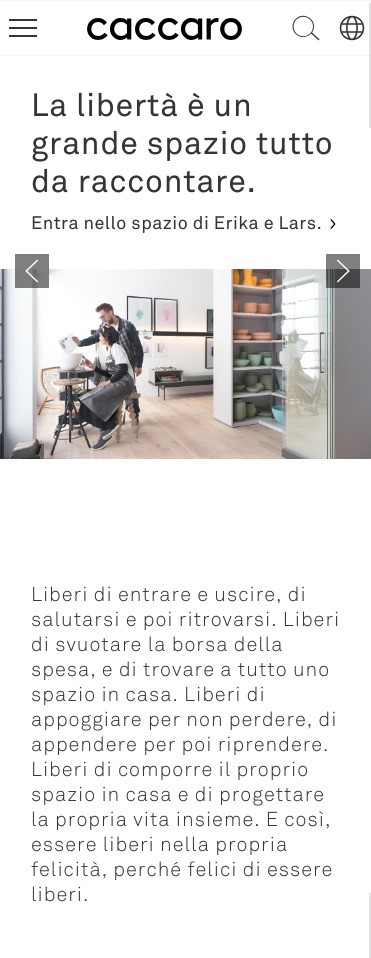
\includegraphics[width=10cm,height=10cm,keepaspectratio]{sez/HomePage/img/mobile-firstcut.jpg}
	\caption{First cut in versione mobile.}
	\label{fig:mobFirstCut}
\end{figure}

\paragraph*{Layout e Immagini}
Netto miglioramento da questo punto di vista. Le immagini occupano molto meno spazio, e vengono messi in primo piano i paragrafi. Vedi \autoref{fig:mobFirstCut}.


\paragraph*{Scrolling}
Seppur meglio sopportato dall'utente in versione mobile, incombe ancora il problema dell'eccessivo scrolling nella homepage.

\paragraph*{Uso con le dita}
Bene l'usabilità del carosello con le immagini a inizio pagina: è possibile scorrere le immagini con degli swipe orizzontali, cosa a cui l'utente è già abituato (si pensi alla galleria presente in ogni smartphone).\\
Bene anche i link, sempre ben spaziati fra di loro. Lo spazio tappabile non è solo il testo stesso, ma si estende anche al di fuori: ottimo, in quanto le dita non hanno la stessa precisione di un mouse (fat finger). Meglio ancora il bottone "Richiedi Cataloghi" (\autoref{fig:mobButton}), che presenta un superficie tappabile ancora maggiore. I collegamenti delle collezioni avrebbero potuto beneficiare di tale design.

\begin{figure}[H]
	\centering
	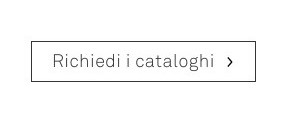
\includegraphics[width=7cm,keepaspectratio]{sez/HomePage/img/mobile-button.jpg}
	\caption[https://www.caccaro.com/]{Bottone ideale per l'uso con le dita.}
	\label{fig:mobButton}
\end{figure}
